

\part{Confronto tra Algoritmi di Ordinamento}

\section{Confronto tra Algoritmi di Ordinamento}

Viene presentato un confronto sulla complessità temporale degli algoritmi principali studiati.

\begin{table}[h]
    \centering
    \renewcommand{\arraystretch}{1.5}
    \begin{tabular}{|l|c|c|c|}
        \hline
        \textbf{Algoritmo} & \textbf{Caso Ottimo} & \textbf{Caso Medio} & \textbf{Caso Pessimo} \\
        \hline
        \textbf{Merge Sort} & $\Theta(n \log n)$ & $\Theta(n \log n)$ & $\Theta(n \log n)$ \\
        \hline
        \textbf{Insertion Sort} & $\Theta(n)$ & $\Theta(n^2)$ & $\Theta(n^2)$ \\
        \hline
        \textbf{Quick Sort} & $\Theta(n \log n)$ & $\Theta(n \log n)$ & $\Theta(n^2)$ \\
        \hline
    \end{tabular}
    \caption{Confronto complessità temporale}
    \label{tab:confronto_algo}
\end{table}

\section{Quick Sort: L'Idea}

L'algoritmo segue l'approccio \textit{"Divide et Impera"} in tre fasi:

\begin{enumerate}
    \item \textbf{Scelta del Perno (Pivot):} Si sceglie un elemento, ad esempio l'ultimo elemento dell'array: $P = A[r]$.
    \item \textbf{Partizione (Partition):} L'array $A$ viene diviso in due metà (non necessariamente uguali) rispetto al pivot:
    \[ A_1 = \{x \in A \mid x \le P\} \]
    \[ A_2 = \{x \in A \mid x > P\} \]
    Il pivot $P$ viene posizionato tra $A_1$ e $A_2$.
    \item \textbf{Ricorsione:} Si ordinano ricorsivamente i sotto-array $A_1$ e $A_2$.
\end{enumerate}

\begin{algorithm}
    \caption{QuickSort(A, p, r)}
    \begin{algorithmic}[1]
        \State \Comment{Goal: Ordina A[p...r]. Prima chiamata: p=1, r=n}
        \If{$p < r$}
            \State $q \gets \textsc{Partition}(A, p, r)$
            \State $\textsc{QuickSort}(A, p, q-1)$
            \State $\textsc{QuickSort}(A, q+1, r)$
        \EndIf
        \State \Comment{\#elementi = $r - p + 1$}
    \end{algorithmic}
\end{algorithm}

\begin{explanation}{Logica QuickSort}
Algoritmo ricorsivo basato su \textit{Divide et Impera}:
\begin{enumerate}
    \item \textbf{Partition}: Trova la posizione finale del pivot $q$.
    \item \textbf{Ricorsione}: Ordina i sotto-array a sinistra e a destra di $q$.
    \item \textbf{Base}: Se $p \ge r$, l'array ha 0 o 1 elemento ed è già ordinato.
\end{enumerate}
\end{explanation}

\section{Confronto: Merge Sort vs Quick Sort}

Entrambi usano la strategia \textit{Divide et Impera}, ma in modo opposto:

\begin{table}[h]
    \centering
    \renewcommand{\arraystretch}{1.5}
    \begin{tabular}{|p{0.15\textwidth}|p{0.38\textwidth}|p{0.38\textwidth}|}
        \hline
        \textbf{Fase} & \textbf{Merge Sort} & \textbf{Quick Sort} \\
        \hline
        \textbf{Divide} & \textbf{Banale:} $q = \lfloor(p+r)/2\rfloor$. Divide a metà perfetta. & \textbf{Complesso:} $q = \textsc{Partition}(\dots)$. Il lavoro "pesante" viene fatto qui. \\
        \hline
        \textbf{Impera} & $\textsc{MS}(A, p, q)$, $\textsc{MS}(A, q+1, r)$ & $\textsc{QS}(A, p, q-1)$, $\textsc{QS}(A, q+1, r)$ \\
        \hline
        \textbf{Combine} & \textbf{Complesso:} $\textsc{Merge}(\dots)$. Necessaria per unire i risultati. & \textbf{Banale:} Non necessaria (l'array è ordinato "in loco"). \\
        \hline
    \end{tabular}
\end{table}

\section{La Procedura Partition}

La funzione \texttt{Partition} riorganizza l'array in loco (senza array di appoggio) in modo lineare $\Theta(n)$.

\begin{algorithm}
    \caption{PARTITION(A, p, r)}
    \begin{algorithmic}[1]
        \State $x \gets A[r]$ \Comment{Pivot}
        \State $i \gets p - 1$
        \For{$j \gets p$ \textbf{to} $r - 1$}
            \If{$A[j] \le x$}
                \State $i \gets i + 1$
                \State \textbf{Swap}($A[i], A[j]$)
            \EndIf
        \EndFor
        \State \textbf{Swap}($A[i+1], A[r]$) \Comment{Posiziona il pivot}
        \State \textbf{return} $i + 1$
    \end{algorithmic}
\end{algorithm}

\begin{explanation}{Partition (Lomuto)}
Scansiona l'array con un indice $j$. Se $A[j] \le Pivot$, incrementa la regione dei "minori" ($i$) e scambia.
Alla fine, il pivot viene messo esattamente tra i minori e i maggiori.
\end{explanation}

\begin{observation}[Invariante del ciclo]
    Durante l'esecuzione, l'array è diviso in regioni:
    \begin{itemize}
        \item $A[p \dots i]$: Elementi $\le$ Pivot.
        \item $A[i+1 \dots j-1]$: Elementi $>$ Pivot.
        \item $A[j \dots r-1]$: Elementi ancora da esaminare.
        \item $A[r]$: Pivot.
    \end{itemize}
\end{observation}

\begin{example}[Traccia Partition]
    \textbf{Array iniziale:} 2 8 7 1 3 5 6 4 (Pivot = 4). \\
    Durante la partizione, gli elementi minori o uguali a 4 vengono spostati a sinistra. Alla fine, il 4 si troverà nella sua posizione corretta definitiva.
\end{example}

\section{Variante: Hoare Partition}

Viene presentata una variante dell'algoritmo di partizione (Partizione di Hoare) che usa due indici che convergono dagli estremi.

\begin{algorithm}
    \caption{HOARE-PARTITION(A, p, r)}
    \begin{algorithmic}[1]
        \State $x \gets A[p]$ \Comment{Pivot (qui preso come primo elemento)}
        \State $i \gets p - 1$
        \State $j \gets r + 1$
        \While{\textbf{true}}
            \Repeat
                \State $j \gets j - 1$
            \Until{$A[j] \le x$}
            \Repeat
                \State $i \gets i + 1$
            \Until{$A[i] \ge x$}
            \If{$i < j$}
                \State \textbf{exchange} $A[i]$ with $A[j]$
            \Else
                \State \textbf{return} $j$
            \EndIf
        \EndWhile
    \end{algorithmic}
\end{algorithm}

\begin{explanation}{Hoare Partition}
Due indici ($i, j$) partono dagli estremi e convergono.
\begin{itemize}
    \item $i$ avanza finché trova elementi "piccoli".
    \item $j$ indietreggia finché trova elementi "grandi".
    \item Quando si bloccano entrambi (trovati elementi fuori posto), si scambiano.
\end{itemize}
È spesso più efficiente di Lomuto in pratica (meno swap).
\end{explanation}
% \end{algorithm} removed duplicate

\section{Analisi della Complessità}

Sia $n = r - p + 1$. Il tempo di esecuzione $T(n)$ dipende da come il pivot divide l'array ($q$).
La relazione di ricorrenza generale è:
$$T(n) = T(q-1) + T(n-q) + \Theta(n)$$
dove $\Theta(n)$ è il costo della Partition.

\subsection{Caso Pessimo}
Si verifica quando l'array è \textbf{già ordinato} (o ordinato al contrario).
In questo caso, il pivot (essendo il massimo o il minimo) divide l'array in un sotto-problema di dimensione $n-1$ e uno di dimensione $0$.
L'albero di ricorsione diventa una lista lunga $n$.

\textbf{Calcolo:}
$$T(n) = T(n-1) + T(0) + c \cdot n$$
Sviluppando la somma:
$$T(n) = \sum_{i=1}^{n} i = \Theta(n^2)$$

\subsection{Caso Ottimo}
Si verifica quando il pivot divide l'array sempre a metà (come nel Merge Sort), ovvero $q = n/2$.
\[ \textbf{Complessità: } O(n \log n) \]

\subsection{Caso Medio}
Anche nel caso medio la complessità si dimostra essere:
\[ O(n \log n) \]

\begin{observation}
    Questo è il motivo per cui il Quick Sort viene utilizzato nella pratica: spesso è più veloce del Merge Sort grazie alle costanti nascoste minori e all'uso della memoria in loco (non richiede array ausiliari per il merge).
\end{observation}



\section*{Quick Sort: Rappresentazione Grafica}

\subsection*{1. L'Idea della Partizione}
L'array viene diviso in due parti (non necessariamente uguali) rispetto a un elemento "perno" (Pivot) $P$.
\begin{itemize}
    \item $A_1$: elementi $\le P$
    \item $A_2$: elementi $> P$
\end{itemize}

\vspace{0.5cm}

\begin{center}
    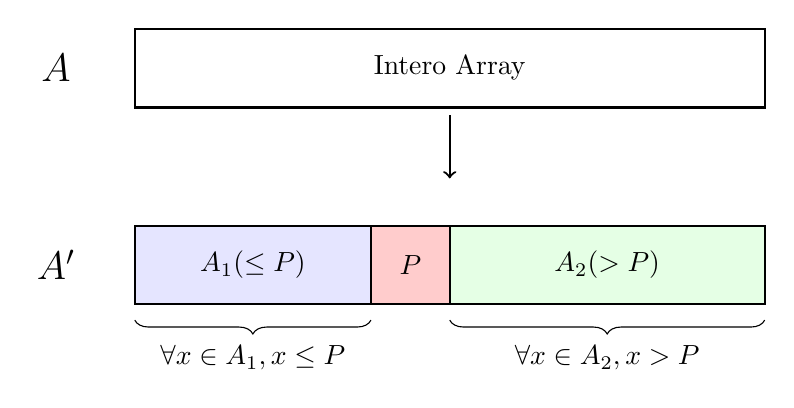
\begin{tikzpicture}
        % Array intero A
        \node at (-1, 1) {\Large $A$};
        \draw[thick] (0, 0.5) rectangle (8, 1.5);
        \node at (4, 1) {Intero Array};

        % Freccia divisione
        \draw[->, thick] (4, 0.4) -- (4, -0.4);

        % Array partizionato
        \node at (-1, -1.5) {\Large $A'$};

        % A1
        \draw[thick, fill=blue!10] (0, -2) rectangle (3, -1);
        \node at (1.5, -1.5) {$A_1 (\le P)$};

        % Pivot
        \draw[thick, fill=red!20] (3, -2) rectangle (4, -1);
        \node at (3.5, -1.5) {$P$};

        % A2
        \draw[thick, fill=green!10] (4, -2) rectangle (8, -1);
        \node at (6, -1.5) {$A_2 (> P)$};

        % Graffe descrizione
        \draw[decorate, decoration={brace, amplitude=5pt, mirror}] (0,-2.2) -- (3,-2.2) node[midway, below=0.2cm] {$\forall x \in A_1, x \le P$};
        \draw[decorate, decoration={brace, amplitude=5pt, mirror}] (4,-2.2) -- (8,-2.2) node[midway, below=0.2cm] {$\forall x \in A_2, x > P$};

    \end{tikzpicture}
\end{center}

\newpage

\subsection*{2. Esempio di Traccia (Partition)}
Esecuzione della partizione sull'array: \texttt{2 8 7 1 3 5 6 4}.
Il Pivot è l'ultimo elemento ($4$).

\vspace{0.5cm}

\begin{center}
    \begin{tikzpicture}[
        cell/.style={rectangle, draw, minimum size=0.8cm, font=\large},
        pivot/.style={rectangle, draw, minimum size=0.8cm, fill=gray!30, font=\large, thick},
        scan/.style={rectangle, draw, minimum size=0.8cm, fill=yellow!20, font=\large},
        swap/.style={rectangle, draw, minimum size=0.8cm, fill=red!20, font=\large}
        ]

        % Funzione per disegnare un passo
        \newcommand{\drawarray}[4]{
        \node[anchor=west] at (-2, 0) {\textbf{#1}};
        \foreach \val [count=\i] in {#2} {
        \pgfmathsetmacro{\x}{(\i-1)*0.8}

        % Stile di default
        \node[cell] (n\i) at (\x, 0) {\val};

        % Evidenzia Pivot (ultima posizione visualizzata come tale)
        \ifnum\i=#3
        \node[pivot] at (\x, 0) {\val};
        \fi
        }
        % Etichette i e j se fornite
        #4
        }

        % Passo 1: Inizio
        \begin{scope}[yshift=0cm]
            \drawarray{Inizio:}{2, 8, 7, 1, 3, 5, 6, 4}{8}{
            \node[below=0.1cm of n8] {\small Pivot};
            \node[above=0.1cm of n1] {$j$};
            \node[above=0.1cm of n1, xshift=-0.8cm] {$i$};
            }
        \end{scope}

        % Passo 2: Trovato 2 <= 4
        \begin{scope}[yshift=-2cm]
            \drawarray{Step 1:}{2, 8, 7, 1, 3, 5, 6, 4}{8}{
            \node[below=0.1cm of n1] {\small $i \gets i+1$};
            \node[draw=none] at (8, 0) {\small (2 $\le$ 4: Swap non nec.)};
            }
        \end{scope}

        % Passo 3: Scansione 8, 7 (maggiori, i fermo)
        \begin{scope}[yshift=-4cm]
            \drawarray{Step 2-3:}{2, 8, 7, 1, 3, 5, 6, 4}{8}{
            \node[above=0.1cm of n1] {$i$};
            \node[above=0.1cm of n3] {$j$};
            \node[draw=none] at (8, 0) {\small (8, 7 $>$ 4: $i$ fermo)};
            }
        \end{scope}

        % Passo 4: Trovato 1 <= 4 -> Swap con A[i+1] (8)
        \begin{scope}[yshift=-6cm]
            \drawarray{Step 4:}{2, 1, 7, 8, 3, 5, 6, 4}{8}{
            \node[swap] at (0.8, 0) {1}; % New pos of 1
            \node[swap] at (2.4, 0) {8}; % New pos of 8
            \node[above=0.1cm of n2] {$i$};
            \node[above=0.1cm of n4] {$j$};
            \draw[<->, thick, red, bend left] (0.8, 0.5) to (2.4, 0.5);
            \node[draw=none] at (8, 0) {\small (1 $\le$ 4: Swap $A[i+1] \leftrightarrow A[j]$)};
            }
        \end{scope}

        % Passo 5: Trovato 3 <= 4 -> Swap con A[i+1] (7)
        \begin{scope}[yshift=-8cm]
            \drawarray{Step 5:}{2, 1, 3, 8, 7, 5, 6, 4}{8}{
            \node[swap] at (1.6, 0) {3};
            \node[swap] at (3.2, 0) {7};
            \node[above=0.1cm of n3] {$i$};
            \node[above=0.1cm of n5] {$j$};
            \draw[<->, thick, red, bend left] (1.6, 0.5) to (3.2, 0.5);
            }
        \end{scope}

        % Passo Finale: Posiziona Pivot
        \begin{scope}[yshift=-10cm]
            \drawarray{Finale:}{2, 1, 3, 4, 7, 5, 6, 8}{4}{
            \node[pivot] at (2.4, 0) {4}; % Pivot in posizione corretta
            \node[above=0.1cm of n4] {Pivot};
            \draw[<->, thick, blue, bend left] (2.4, 0.5) to (5.6, 0.5);
            \node[draw=none] at (8, 0) {\small (Swap $A[i+1] \leftrightarrow A[r]$)};
            }
        \end{scope}

    \end{tikzpicture}
\end{center}

\newpage

\subsection*{3. Invariante della Procedura Partition}
Durante la scansione, l'array è diviso in 4 regioni dinamiche gestite dagli indici $i$ e $j$.

\vspace{1cm}

\begin{center}
    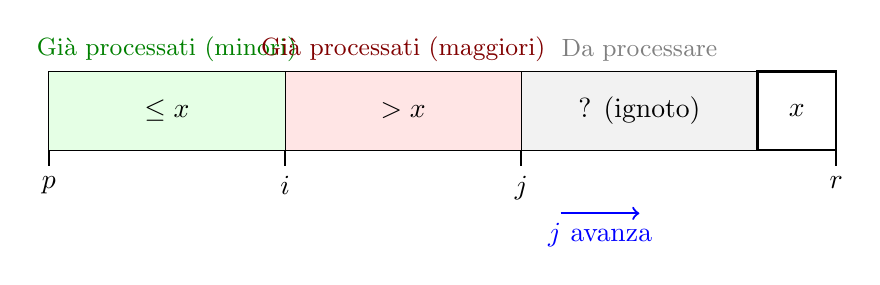
\begin{tikzpicture}[scale=1.0]
        % Definizioni dimensioni
        \def\h{1} % Altezza celle

        % Regioni
        % Regione <= x
        \draw[fill=green!10] (0,0) rectangle (3,\h);
        \node at (1.5, 0.5) {$\le x$};

        % Regione > x
        \draw[fill=red!10] (3,0) rectangle (6,\h);
        \node at (4.5, 0.5) {$> x$};

        % Regione da esaminare
        \draw[fill=gray!10] (6,0) rectangle (9,\h);
        \node at (7.5, 0.5) {? (ignoto)};

        % Pivot
        \draw[thick] (9,0) rectangle (10,\h);
        \node at (9.5, 0.5) {$x$};

        % Indici sotto
        \draw[thick] (0,0) -- (0,-0.2) node[below] {$p$};
        \draw[thick] (3,0) -- (3,-0.2) node[below] {$i$};
        \draw[thick] (6,0) -- (6,-0.2) node[below] {$j$};
        \draw[thick] (10,0) -- (10,-0.2) node[below] {$r$};

        % Descrizione sopra
        \node[above, font=\small, text=green!50!black] at (1.5, \h) {Già processati (minori)};
        \node[above, font=\small, text=red!50!black] at (4.5, \h) {Già processati (maggiori)};
        \node[above, font=\small, text=gray] at (7.5, \h) {Da processare};

        % Loop
        \draw[->, thick, blue] (6.5, -0.8) -- (7.5, -0.8) node[midway, below] {$j$ avanza};

    \end{tikzpicture}
\end{center}

\newpage

